\chapter{Introducci\'on}\label{CAP:Introduccion}
En este cap\'itulo se introduce al lector poco a poco en lo que tratar\'a esta memoria, las aplicaciones web de nuestros d\'ias y c\'omo han evolucionado a lo largo de los tiempos.\\

\section{Motivaci�n}\label{SEC:Seccion1}
En este proyecto se han querido combinar las funcionalidades de la Web 2.0 con la idea en la que se mueve Facebook y crear una aplicaci\'on web para la interacci\'on entre alumnos Erasmus y ex alumnos Erasmus. La finalidad que persigue es ayudar a resolver las dudas que les puedan surgir a los futuros alumnos Erasmus. Existen adem\'as multitud de herramientas online que nos ofrecen todo tipo de informaci\'on necesaria para las estancias erasmus, pero ninguna espec\'ificamente para la escuela.\\

\subsection{TuErasmus}
Esta web constituir\'a un apoyo para todo aquel que se encuentre frente a numerosas preguntas sobre qu\'e hacer cuando comience la aventura Erasmus, qu\'e cosas tener en cuenta, d\'onde poder alojarse, qu\'e es necesario hacer antes de ir a las ciudades destino... En ella podr\'an encontrar las respuestas a todas las preguntas que les ir\'an surgiendo a lo largo del proceso de preparaci\'on de su experiencia Erasmus. Adem\'as se incluir\'a un apartado donde antiguos alumnos Erasmus compartir\'an sus experiencias, rutas tur\'isticas, consejos, advertencias de convivencia... para conseguir que otros alumnos tengan una mejor experiencia.\\

\begin{figure}[htbp]
	
	\centering
	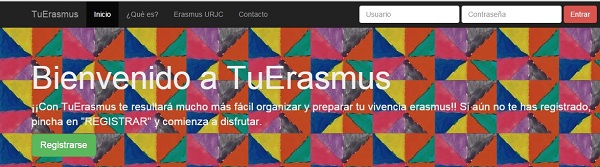
\includegraphics[scale=0.5]{./Figuras/tuerasmus.jpg}
	\caption{Aplicaci\'on web "TuErasmus". }
	\label{fig:webs20}
	
\end{figure}

\section{Becas Erasmus}\label{SEC:Seccion2}

\subsection{�Qu� es Erasmus?}
El programa ERASMUS, \textit{EuRopean Comunity Action Scheme for the Mobility of University Students}, es un plan de gesti\'on de distintas administraciones p\'ublicas que permite la movilidad acad\'emica de los estudiantes y profesores por los pa\'ises que forman la Uni\'on Europea, el Espacio Econ\'omico Europeo, Suiza y Turqu\'ia. Est\'a orientado a la ense\~nanza superior, y su objetivo es la mejora de la calidad y fortalecer la dimensi\'on europea de la ense�anza superior fomentando la cooperaci\'on transnacional entre universidades, estimulando la movilidad en Europa y mejorando la transparencia y el pleno reconocimiento acad\'emico de los estudios y cualificaciones en toda la Uni\'on.\\

\subsection{�Qu� hacer?}
Para poder optar a la beca Erasmus solo se requiere estar cursando una carrera universitaria superior (grado o m�ster) y haber completado el primer a\~no de formaci\'on, y ser ciudadano de alguno de los estados que est\'an asociados al programa S\'ocrates\footnote[1]{El programa S\'ocrates es un programa de la Uni\'on Europea adoptado en junio de 1997 para la cooperaci\'on en el \'ambito de la educaci\'on. El cap\'itulo de S\'ocrates dedicado a la ense�anza superior es Erasmus. A trav\'es de esta acci\'on las universidades reciben ayudas financieras, con el fin de fomentar el intercambio de estudiantes y profesores, y la cooperaci\'on en la ense\~nanza superior de los pa\'ises de la UE y los pa\'ises asociados (Noruega, Islandia, Liechtenstein, Eslovaquia, Chipre, Hungr\'ia, Polonia, Ruman\'ia, Chequia, Letonia, Estonia, Lituania, Bulgaria y Eslovenia).}.\\ 

Aquellos alumnos que cumplan los requisitos y hayan sido seleccionados para dicho programa, cursar\'an sus estudios durante un periodo de tiempo comprendido entre tres y doce meses.\\

\subsection{La experiencia Erasmus}
El programa Erasmus brinda a numerosos estudiantes la oportunidad de poder vivir por primera vez en un pa\'is extranjero. Es por ello que actualmente este programa supone un importante fen\'omeno social y cultural para los estudiantes universitarios. Es as\'i, que algunos escritores o guionistas se han inspirado en ello para la creaci\'on de sus libros y pel\'iculas.\\

El programa favorece el aprendizaje y el entendimiento de culturas y costumbres distintas a las de nuestros propios pa\'ises, adem\'as de ayudar a entender mucho mejor el sentido de comunidad entre los estudiantes de distintas nacionalidades. Esta experiencia Erasmus se considera, igualmente, como una etapa de aprendizaje y de impulso de la vida social. A lo largo de la experiencia Erasmus, los estudiantes son testigos de multitud de eventos, como por ejemplo las fiestas Erasmus, que se celebran en las ciudades anfitrionas y son conocidas por ser ruidosas y multiling�es, quedadas Erasmus, clases de apoyo, viajes...\\

Con el paso de los a�os el programa Erasmus se est\'a haciendo m\'as importante, y siendo cada vez m\'as primordial en el mundo acad\'emico europeo e incluso en la vida social de los estudiantes, permitiendo en numerosas ocasiones el nacimiento de nuevas amistades, llegando algunas a traspasar fronteras e incluso a perdurar tanto o m\'as que otras amistades que comienzan desde nuestras \'epocas de preescolar. Como cada vez hay m\'as estudiantes universitarios, comienzan a surgir las generaciones Erasmus, para distinguir a esos estudiantes. El programa de intercambio Erasmus de la Uni\'on Europea ha sido galardonado con el Premio Pr\'incipe de Asturias de Cooperaci\'on Internacional 2004 por ser uno de los programas de intercambio cultural m\'as importante de la historia de la humanidad.\\

\section{Web 2.0}\label{SEC:Seccion3}
Desde que surgi\'o la web hasta hoy en d\'ia, \'esta ha experimentado una notable transformaci\'on, tanto en la forma en que es desarrollada como en la forma en que los usuarios hacen uso de ella. Por otro lado, los lenguajes de programaci\'on empleados para desarrollar p\'aginas web han ido evolucionando, permitiendo la creaci\'on de p\'aginas cada vez m\'as ligeras, activas, y atractivas. Los usuarios han ido notando que ahora van teniendo m\'as y m\'as control sobre ellas.\\

\begin{figure}[htbp]
	
	\centering
	
\includegraphics[scale=0.5]{./Figuras/web20.jpg}
	\caption{Web 2.0. }
	\label{fig:webs20}
	
\end{figure}

\subsection{De las Web 1.0 a las Web 2.0}
El concepto Web 2.0 se refiere a una segunda generaci\'on web basada en comunidades de usuarios y una gama especial de servicios redes sociales, blogs, wikis, etc. de tecnolog\'ia diferente, donde los cambios se
producen en la forma en la que los desarrolladores de software y los usuarios finales acceden a la red. En general, cuando mencionamos el t\'ermino Web 2.0 nos referimos a una serie de aplicaciones y p\'aginas de Internet que utilizan la inteligencia colectiva para proporcionar servicios interactivos en red dando al usuario el control de sus datos.\\

En s\'intesis, la Web 2.0 es la representaci\'on de la evoluci\'on de las aplicaciones tradicionales hacia aplicaciones web enfocadas al usuario final; una actitud y no precisamente una tecnolog\'ia; un sitio web que permite a sus usuarios interactuar con otros usuarios o cambiar contenidos del sitio a diferencia de otros sitios web no interactivos donde los usuarios se limitan a la visualizaci\'on pasiva de informaci\'on.\\

\subsection{Web 1.0 vs Web 2.0}
En las Web 1.0 encontramos la informaci\'on centralizada, sitios con contenidos de alta y baja calidad administrados por un webmaster, informaci\'on poco actualizada, software tradicionales, contenidos y sitios m\'as bien est\'aticos, dise\~no y producci\'on a cargo de quienes conocen sobre inform\'atica, sitios con fines generalmente comerciales, y cuyo objetivo es difundir informaci\'on.\\

Por el contrario, en las Web 2.0 la informaci\'on est\'a descentralizada, hay una amplia diversidad en contenidos administrados por usuarios, informaci\'on en permanente cambio, software y aplicaciones que no requieren de su instalaci\'on en el PC para utilizarlos, contenidos y sitios flexibles en cont\'inua transformaci\'on, dise\~no y producci\'on en necesidad de grandes conocimientos de inform\'atica, sitios con fines diversos, en la mayor\'ia de los casos, la construcci\'on de comunidades que comparten intereses, y cuyo objetivo es producir, dise\~nar, construir y compartir informaci\'on.\\

En las \textbf{Web 1.0} el modo de interactuar es mediante lectura; la experiencia y expectativa de los usuarios es navegar y consumir, MB de textos y fotos publicados. El usuario suele ser un consumidor pasivo, la principal actividad es \textit{Downloading}, la tecnolog�a se usa para crear p\'aginas est\'aticas con un webmaster editor, y el periodo de estas web comprende desde 1994 a 2004.\\

En las \textbf{Web 2.0} el modo de interactuar es mediante lectura y escritura; la experiencia y expectativa de los usuarios es conectar, colaborar, crear, compartir. Ya no tenemos MB, sino que tenemos GB de v\'ideo y audio compartidos. El usuario suele ser un participante activo, la actividad principal es \textit{Uploading}, la tecnolog\'ia se aplica para crear p\'aginas din\'amicas, todos los software editan, no hay que tener ninguno espec�fico. El periodo de estas nuevas web comprende desde 2004 hasta la actualidad, aunque poco a poco comencemos a o\'ir el concepto \textbf{Web 3.0}, que ser\'a la pr\'oxima generaci\'on de p\'aginas din\'amicas.\\

\section{Herramientas colaborativas}
Las herramientas colaborativas son los sistemas que permiten acceder a ciertos servicios que facilitan a los usuarios comunicarse y trabajar conjuntamente sin importar que no est\'en reunidos en un mismo lugar f\'isico. En general, con ellas se puede compartir informaci\'on en determinados formatos (audio, texto, v\'ideo).\\

Para la creaci\'on de estas Web 2.0 existen multitud de herramientas online. Muchas de ellas pueden ser colaborativas (aunque no todas); lo importante para ello es conocerlas y ver si nos pueden servir como herramientas de car\'acter colaborativo.\\

\section{Estructura de la memoria}\label{SEC:Seccion4}
Esta memoria se divide en cuatro grandes bloques: estado del arte, dise\~no e implementaci\'on de la aplicaci\'on web, despliegue y pruebas, y conclusiones finales. En el segundo cap\'itulo, \textit{\nameref{CAP:Estadodelarte}} se har� una introducci�n sobre cada una de las distintas tecnolog\'ias utilizadas en el proyecto; en el tercer cap\'itulo, \textit{\nameref{CAP:Disenoimplementacion}} hablaremos sobre las distintas etapas del desarrollo e implementaci\'on de la aplicaci\'on web, as\'i como alguna menci\'on a las dificultades encontradas durante el proceso; en el cuarto cap\'itulo, \textit{\nameref{CAP:Despliegueyresultados}} haremos un breve resumen sobre las pruebas realizadas y los resultados obtenidos; y por \'ultimo, en el quinto cap\'itulo, \textit{\nameref{CAP:Conclusiones}} encontraremos todo lo relacionado a las conclusiones finales que hemos obtenido tras la realizaci�n del proyecto, y posibles l\'ineas futuras.\\
